% Szglab4
% ===========================================================================
%
\chapter{Szkeleton tervezése}

\thispagestyle{fancy}

\section{A szkeleton modell valóságos use-case-ei}


\subsection{Use-case diagram}

\begin{figure}[h]
\begin{center}
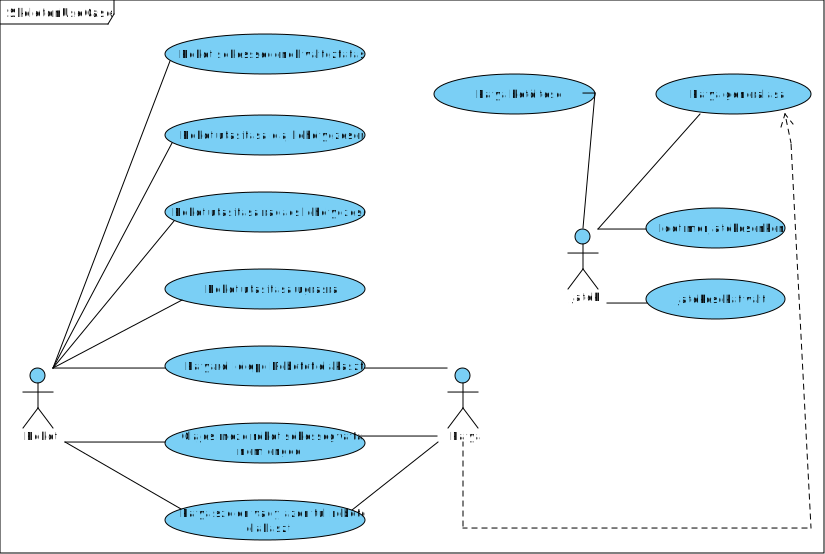
\includegraphics[width=\textwidth]{chapters/chapter05/SkeletonUseCase.pdf}
\caption{Szkeleton Use Case Diagram}
\label{fig:SzkeletonUseCase}
\end{center}
\end{figure}

\subsection{Use-case leírások}
%\comment{Minden use-case-hez külön}

\usecase%
{Új játék indítása}%
{Elindíthatunk egy új játékot}%
{Játékos, Játék}%
{A játékosok számának megadása után a Játékos kezdeményezheti a játéknak az elindítását}

\usecase%
{Időt mér játékosonkét}%
{Játékmenet és Játékosonkénti időnyilvántartás}%
{Játék}%
{Nyilvántartja a Játékosok még hátralévő idejét, és megállítja azokat akik már nem képhetnek}

\usecase%
{Játékosokat vált}%
{Játékosokat vált körönként}%
{Játék}%
{Játékost cserél körönként ha a játékos ugrott vagy lejárt az ideje}

\usecase%
{Robot sebességének változtatása}%
{A Játékos megváltoztathatja a Robotnak a sebességét}%
{Játékos, Robot}%
{A játékos körönként megváltoztathatja a Robotnak a sebességét}

\usecase%
{Robot utasítása olajnak a lehelyezése}%
{Játékos utasíthatja a Robotot, hogy helyezze le az olajfoltot}%
{Játékos, Robot}%
{A Játékos más játékosok hátráltatásának okán lehelyezhet a készletáéből egy olajfoltot}

\usecase%
{Robot utasítása ragacsnak a lehelyezése}%
{Játékos utasíthatja a Robotot, hogy helyezze le az ragacsfoltot}%
{Játékos, Robot}%
{A Játékos más játékosok hátráltatásának okán lehelyezhet a készletáéből egy ragacsfoltot}

\usecase%
{Robot utasítása ugrásra}%
{Játékos utasíthatja a Robotot, hogy végezze el az ugrást}%
{Játékos, Robot, Játék}%
{Játékos utasíthatja a Robotot, hogy végezze el az ugrást, amennyiben ezt nem teszi meg a Játék kikényszerítheti ezt a lépést}

\usecase%
{Olajos mező Robot sebességváltoztatást nem enged}%
{Ha olajos mezőn vagyunk akkor a mező nem engedi a lépést a robotnak}%
{Robot, Pálya}%
{Ha egy Robot rálép az olajra akkor a mező nem engedi neki a sebességváltoztatást}

\usecase%
{Ragacs mező Robot sebességet megfelez}%
{Ha ragacsos mezőn vagyunk akkor a mező megfelezi a Robot sebességét}%
{Robot, Pálya}%
{Ha egy Robot rálép a ragacsra akkor a mező megfelezi aa Robotnak a sebességét}

\usecase%
{Pályáról lelépő Robotot elakaszt}%
{Pályáról lelépő robotot elakasztjuk, nem léphet tovább}%
{Robot, Pálya}%
{Ha egy Robot kilép a pálya határain kívülre akkor elakasztja őt}

\section{A szkeleton kezelői felületének terve, dialógusok}
A szkeleton menüvezérléssel teszi lehetővé a különböző funckiók tesztelését. Egy teszt futtatásához szükséges a felhsználónak
megadni a tesztesetet, melyet futtatni kíván. 

A menü felépítése: \\

Példa:
1. [Use-case neve] \\
1.1 [Teszteset neve][Visszatérése] \\
1.2 [Teszteset neve][Visszatérése] \\
1.3 [Teszteset neve][Visszatérése] \\
   1.3.1 [Teszteset neve][Visszatérése] \\
... \\

Az egyes tesztesetek nevei az első pontban leírt use-casek. A tesztesetek pedig
az adott use-case összes szekvenciáját végrehajtják, amennyiben azt a felhasználó igényli. \\

A kimenet felépítése: \\

Példa: \\

Adja meg a végrehajtandó Use-case számát: X \\
X. [Use-case neve] \\
>   <osztály::függvénynév(paraméter)> \\
>         <osztály::függvénynév(paraméter)> \\
>               <osztály::függvénynév(paraméter)> \\
.                    [Teszteset neve][Értéke] \\
<               <osztály::függvénynév(paraméter)> \\
<         <osztály::függvénynév(paraméter)> \\
<   <osztály::függvénynév(paraméter)> \\

A fenti példában a > szimbólum jelzi egy függvény meghívását, < pedig egy függvény
visszatérését. A . szimbólum valamely teszteset lefutását mutatja, mely után annak 
visszatérési értéke is látszik, jelezvén, hogy sikeresen lefutott-e. \\


\clearpage
\section{Szekvencia diagramok a belső működésre}

A korábbi fejezetben lévő szekvencia diagramok továbbra is érvényesek.

\begin{figure}[h]
	\begin{center}
		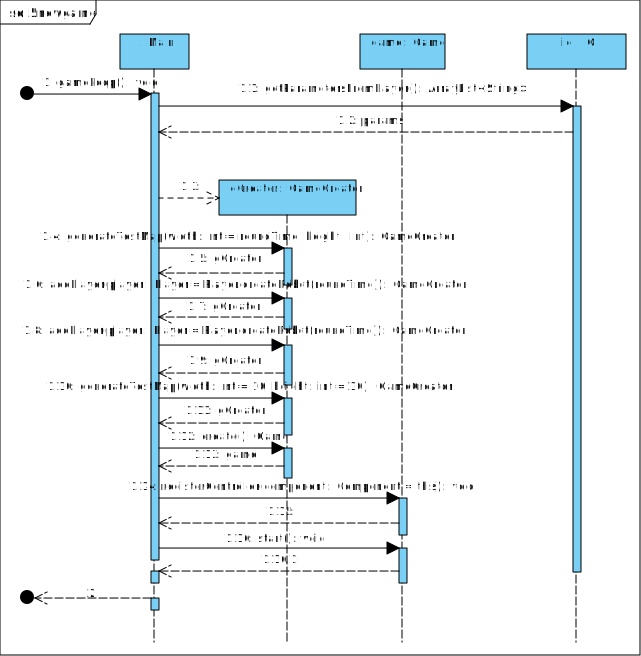
\includegraphics[width=\textwidth]{chapters/chapter05/5newgame.pdf}
		\caption{Új játék indítása, paraméterek megadása}
		\label{fig:5newgame}
	\end{center}
\end{figure}


\begin{figure}[h]
	\begin{center}
		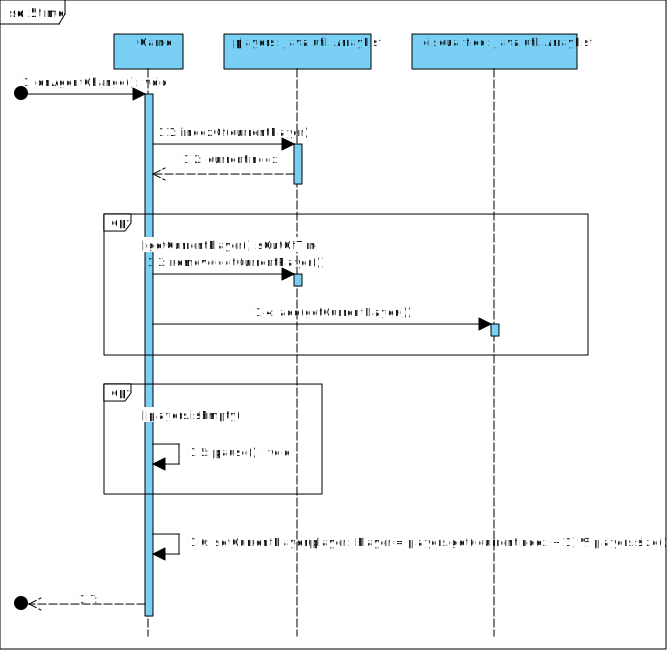
\includegraphics[width=\textwidth]{chapters/chapter05/5time.pdf}
		\caption{Idő nyilvántartása és a játékosok léptetése}
		\label{fig:5time}
	\end{center}
\end{figure}
\clearpage

\begin{figure}[h]
    \begin{center}
        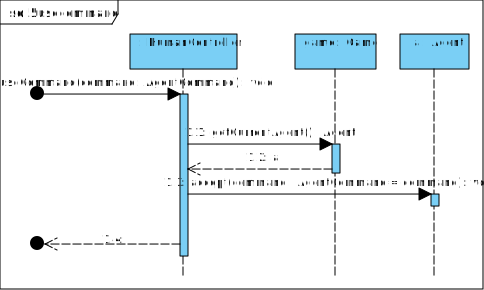
\includegraphics[width=\textwidth]{chapters/chapter05/5usecommand.pdf}
        \caption{Command küldése Agentnek}
        \label{fig:5usecommand}
    \end{center}
\end{figure}
\clearpage

\begin{figure}[h]
    \begin{center}
        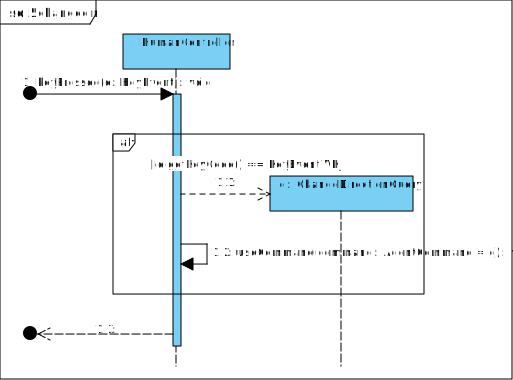
\includegraphics[width=\textwidth]{chapters/chapter05/5changedir.pdf}
        \caption{Robot utasítása irány változtatásra}
        \label{fig:5changedir}
    \end{center}
\end{figure}
\clearpage

\begin{figure}[h]
    \begin{center}
        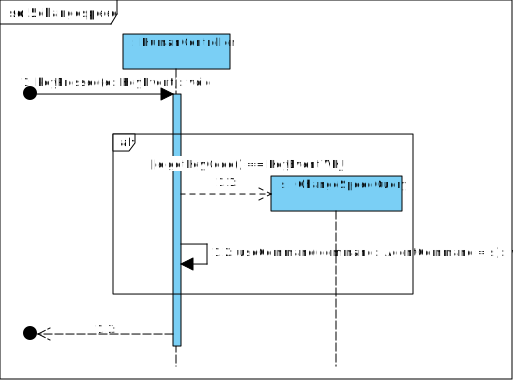
\includegraphics[width=\textwidth]{chapters/chapter05/5changespeed.pdf}
        \caption{Robot utasítása sebesség változtatásra}
        \label{fig:5changespeed}
    \end{center}
\end{figure}
\clearpage

\begin{figure}[h]
    \begin{center}
        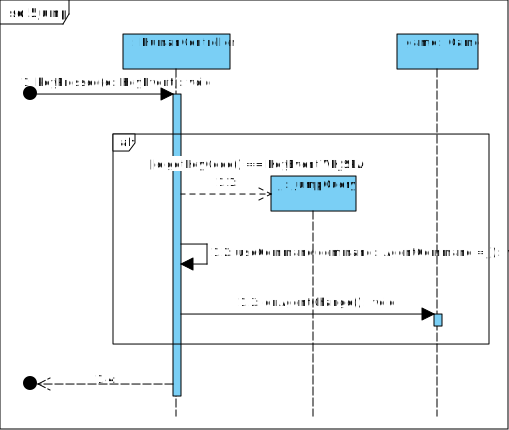
\includegraphics[width=\textwidth]{chapters/chapter05/5jump.pdf}
        \caption{Robot utasítása ugrásra}
        \label{fig:5jump}
    \end{center}
\end{figure}
\clearpage

\begin{figure}[h]
    \begin{center}
        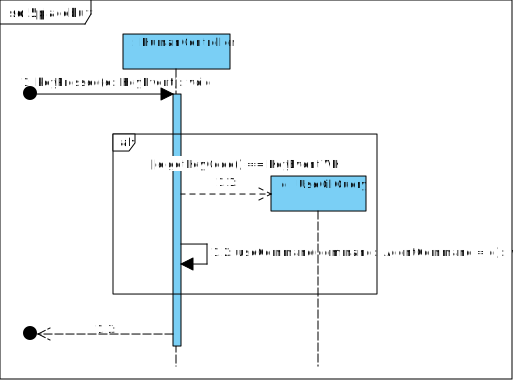
\includegraphics[width=\textwidth]{chapters/chapter05/5placebuff.pdf}
        \caption{Robot utasítása buff lehelyezésére}
        \label{fig:5placebuff}
    \end{center}
\end{figure}
\clearpage

\section{Kommunikációs diagramok}


\begin{figure}[h]
	\begin{center}
		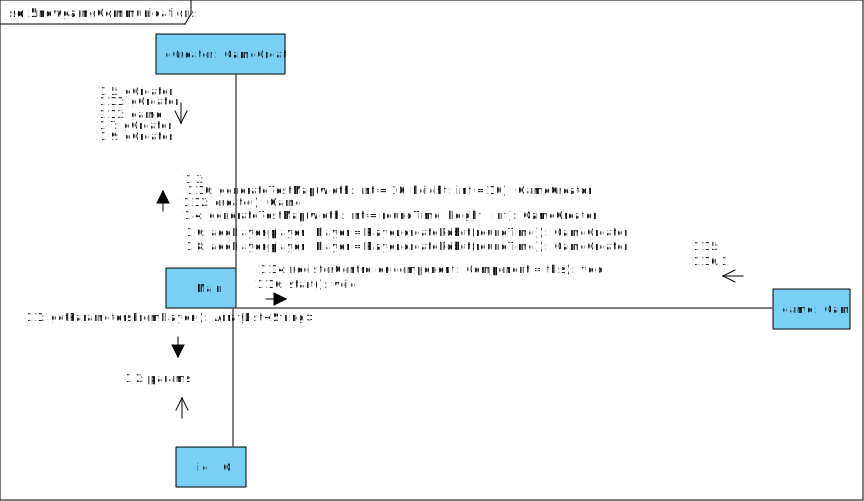
\includegraphics[width=\textwidth]{chapters/chapter05/5newgameCommunications.pdf}
		\caption{Új játék indítása, paraméterek megadása}
		\label{fig:5newgameCommunication}
	\end{center}
\end{figure}

\begin{figure}[h]
	\begin{center}
		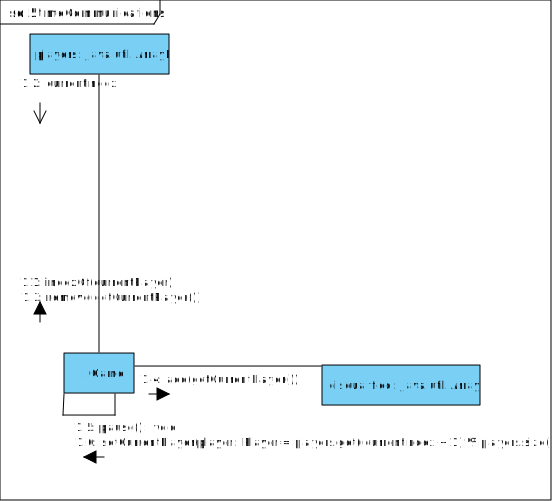
\includegraphics[width=\textwidth]{chapters/chapter05/5timeCommunications.pdf}
		\caption{Idő nyilvántartása és a játékosok léptetése}
		\label{fig:5timeCommunication}
	\end{center}
\end{figure}

\begin{figure}[h]
	\begin{center}
		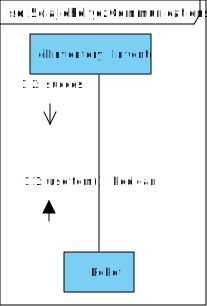
\includegraphics[width=\textwidth]{chapters/chapter05/5olajlehelyezCommunications.pdf}
		\caption{Robot utasítása olajnak a lehelyezésére}
		\label{fig:5robotolajlehelyezCommunication}
	\end{center}
\end{figure}

\begin{figure}[h]
	\begin{center}
		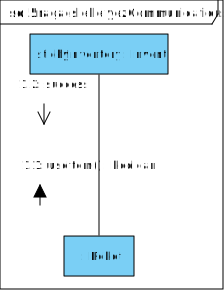
\includegraphics[width=\textwidth]{chapters/chapter05/5ragacslehelyezCommunications.pdf}
		\caption{Robot utasítása ragacsnak a lehelyezésére}
		\label{fig:5robotragacslehelyezCommunication}
	\end{center}
\end{figure}

\begin{figure}[h]
	\begin{center}
		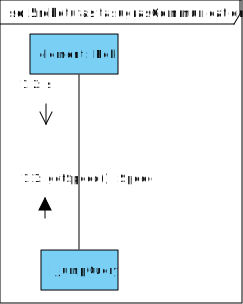
\includegraphics[width=\textwidth]{chapters/chapter05/5robotutasitasugrasCommunications.pdf}
		\caption{Robot utasítása ugrásra}
		\label{fig:5robotutasitugrasCommunication}
	\end{center}
\end{figure}

\begin{figure}[h]
	\begin{center}
		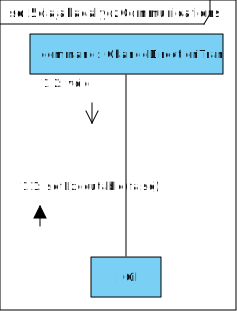
\includegraphics[width=\textwidth]{chapters/chapter05/5olajakadalyozCommunications.pdf}
		\caption{Olajos mező Robot sebességváltoztatást nem enged}
		\label{fig:5olajakadalyozCommunication}
	\end{center}
\end{figure}

\begin{figure}[h]
	\begin{center}
		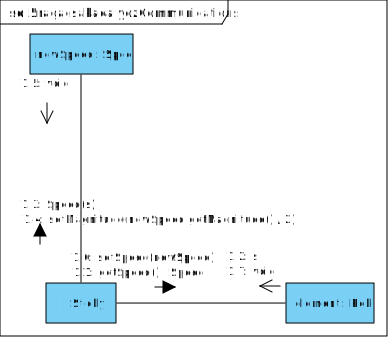
\includegraphics[width=\textwidth]{chapters/chapter05/5ragacsakadalyozCommunications.pdf}
		\caption{Ragacs mező Robot sebességet megfelez}
		\label{fig:5ragacsakadalyozCommunication}
	\end{center}
\end{figure}

\clearpage

